
%%=============================================================================
%% Inleiding
%%=============================================================================

\chapter{Inleiding}
\label{ch:inleiding}

“The full Safari engine is inside of iPhone. And so, you can write amazing Web 2.0 and Ajax apps that look exactly and behave exactly like apps on the iPhone. And these apps can integrate perfectly with iPhone services. They can make a call, they can send an email, they can look up a location on Google Maps. And guess what there is no SKD that you need. You got everything you need if you know how to write apps using the most modern web standards to write amazing apps for the IPhone today” ~\autocite{keynote2007}

Steve Jobs schetste in zijn speech in 2007 al een idee omtrent wat we tegenwoordig progressive web apps ofwel PWA's noemen. Hierbij stelde hij Apple's internetbrowser Safari voor waarop hij een idee gaf wat er allemaal mogelijk mee is. In 2008 introduceerde Apple de App Store waardoor het idee rond progressive web apps meer op de achtergrond raakte.

De voorbije jaren zijn er 3 grote spelers op de mobiele markt geweest, Apple, Windows en Android. Elk van deze hebben hun eigen store waar ze apps aanbieden en waar je als ontwikkelaar je apps op kunt lanceren. Elke store werkt met een eigen programmeertaal.
\begin{itemize}  
	\item Android: Java
	\item Apple: Recent overgeschakeld van Objective-C naar Swift
	\item Windows: C\#
\end{itemize}

Je hoeft natuurlijk niet je app op de store te plaatsen. Je kan dit ook aanbieden op je eigen website. Hiervoor moeten gebruikers je APK downloaden en installaren. Een 'Android Package Kit' of APK is de bestandsextensie die gebruikt wordt door het besturingssysteem van Android voor hun mobiele apps. Net zoals Windows .exe bestanden heeft gebruikt Android .apk ~\autocite{apk}

Als ontwikkelaar wil je geen 3 verschillende programmeertalen leren. Als bedrijf wil je niet 3 verschillende mensen huren voor hetzelfde werk te doen.

Als antwoord hierop heeft Google op de "Google I/O, the developer conference" PWA's voorgesteld. Progressive web apps. Google beschrijft de progressive web app als "applicaties die gebruik maken van nieuwe technologiën om zo het beste van native apps en mobiele website naar de gebruiker te brengen. Ze zijn betrouwbaar en snel".
Met andere woorden, Google wilt webapplicaties die de voordelen van native apps gaan gebruiken zodat de webapp zich gaat gedragen als een native app. 
Als ontwikkelaar zou je dan eenmaal je webapp moeten maken en kan deze op eender welk platform bekeken en gebruikt worden. Je zou geen verschillende programmeertalen moeten leren om dit voor elk platform apart te maken en toch zal het op elk platform lijken alsof het een native app is, speciaal gemaakt voor Android, Apple, ...






\section{Stand van zaken}
\label{sec:stand-van-zaken}

%% TODO: deze sectie (die je kan opsplitsen in verschillende secties) bevat je
%% literatuurstudie. Vergeet niet telkens je bronnen te vermelden!
Voordat we kunnen gaan kijken wat nu het beste alternatief is moeten we eerste begrijpen wat nu juist een PWA is en wat een native app is.

\subsection{Wat is een native app}
Een native mobile app is een applicatie voor op de smartphone die gemaakt is voor gebruik op een specifiek platform in een specifieke programmeertaal ~\autocite{mobileWat}. Doordat een app specifiek voor dat platform gemaakt is kan de app gebruik maken van enkele interne technologiën van de smartphone zoals GPS, bluetooth, camera,... Een goed voorbeeld hierbij is Pokemon Go. Pokemon Go maakt gebruik van vele verschillende functionaliteiten van je smartphone. Het gaat je camera gebruiken voor de pokemons weer te geven in de echte wereld, je GPS gebruiken om te weten waar je bent, meten hoe snel je gaat, ...  Doordat Pokemon Go een native app is die speciaal gemaakt is voor het platform waarop het draait, dit kan zowel Apple als Android zijn, krijgt het de mogelijkheid om deze functionaliteiten te gebruiken. 

Een ontwikkelaar die een native app maakt gaat afhankelijk van het platform een andere programmeertaal moeten gebruiken. Eenmaal zijn app geschreven is kan hij deze door gebruikers laten downloaden. Hij kan dit aanbieden op zijn eigen site via de apk ofwel via de store. Na installatie worden gegevens op de mobiele telefoon opgeslaan. De gebruiker kan nadien de app gebruiken zonder deze opnieuw te moeten installaren. (zie overzicht \ref{table:webVsNative}).


% first column
\begin{minipage}[t]{0.5\textwidth}
	\textbf{Voordelen}
	\begin{itemize}  
		\item Maximaal gebruik van alle functionaliteiten van het apparaat (camera, GPS, \dots)
		\item Geen internetverbinding nodig
		\item Integratie mogelijkheden met andere apps
		\item Hogere snelheid op het apparaat
	\end{itemize}
\end{minipage}
%second column
\begin{minipage}[t]{0.5\textwidth}
		\textbf{Nadelen}
	\begin{itemize}  
		\item Per platform moet apart ontwikkeld worden
		\item Goedkeuring voor plaatsing in de store
		\item Updates in software van het platform (bv. na een update van Android) is het mogelijk dat de app moet worden aangepast
\end{itemize}
\end{minipage}


\subsection{Wat is een web app}
Steeds meer en meer worden websites mobiel bezocht. In 2017 werden 37\% van de websites bezocht via desktop en 63\% mobiel.(\ref{fig:visitsWeb}) Gebaseerd op deze gegevens lijkt het waarschijnlijk dat aan het einde van 2018 66\% van alle bezoeken op websites via de mobiele telefoon zal zijn. ~\autocite{traffic}. Hierdoor is het dus belangrijk dat je je website optimaliseert voor mobiel gebruik. Een website die hiervoor is geoptimaliseerd is een webapp. Webapps moeten altijd bezocht worden via de browser. De gebruiker gaat naar zijn favoriete internetbrowser en kan via de link de webapp opzoeken en bezoeken. Webapps hoeven dus niet geïnstalleerd te worden. Met behulp van een bladwijzer kan een koppeling gemaakt worden op home-scherm van je apparaat. (zie overzicht \ref{table:webVsNative}).


% first column
\begin{minipage}[t]{0.5\textwidth}
	\textbf{Voordelen}
	\begin{itemize}  
		\item Doordat het een webapp is, is het niet platformafhankelijk. 
		\item Makkelijk te delen. Je deelt gewoon een link en de gebruiker moet niets installeren
		\item Gebruikers zien altijd de laatste versie zonder updates te hoeven downloaden van de app.
	\end{itemize}
\end{minipage}
%second column
\begin{minipage}[t]{0.5\textwidth}
	\textbf{Nadelen}
	\begin{itemize}  
		\item Het kan niet alle functionaliteiten van je apparaat gebruiken
		\item Een webapp is niet vindbaar in de store
	\end{itemize}
\end{minipage}


\subsection{Web vs Native}
Uit een onderzoek \textcite{comScore} in 2016 is gebleken  dat gebruikers 87\% van hun tijd op de smarthphone of tablet doorbrengen op een mobiele app terwijl ze maar 13\% van hun tijd doorbrengen op het web. Als je deze cijfers ziet zou je je kunnen afvragen of het wel slim is je tijd te investeren in een web app. Is het niet beter je tijd te spenderen aan het ontwikkelen van native apps? Je hebt miscchien wat meer werk om het op elk platform apart te kunnen krijgen maar als je cijfers ziet van de gebruikers lijkt het erop dat het wel zijn vruchten kan afwerpen.
(zie figuur \ref{fig:usage}). 

Ondanks dat de gebruiker gemiddeld meer tijd doorbrengt op een native app zien we in hetzelfde onderzoek van \textcite{comScore}  dat de helft van alle gebruikers maar 1 app per maand download. Dit is een zeer laag nummer als je weet dat er in het eerste kwartaal van 2018 ongeveer 7.133.500 apps beschikbaar waren over de verschillende stores. Als je enkel kijkt naar degenen die wel apps downloaden merk je dat deze gemiddeld 3,5 apps per maand downloaden. Meer dan de helft van deze apps wordt gedownload door 13\% van de smartphone eigenaars. (zie figuur \ref{fig:downloads}).

Dit komt doordat, ondanks gebruikers meer tijd spenderen op apps dan op mobiele websites, er maandelijks meer unieke gebruikers zijn die gebruik maken van een website dan van een app. (zie figuur \ref{fig:visitors} ) Hieruit kunnen we concluderen dat gebruikers weliswaar meer tijd doorbrengen op apps maar dat ze wel online actiever bezig zijn. Gebruikers gaan niet zoveel nieuwe apps downloaden maar wel veel tijd doorbrengen op hun favoriete app. Gemiddeld brengen gebruikers 45\% van hun tijd door op hun favoriete app en 75\% met hun top 3 apps (zie figuur \ref{fig:timeSpent}).

Als je een native app hebt heb je veel concurrenten. Het is moeilijk om veel gebruikers te krijgen aangezien maar weinigen nieuwe apps downloaden. Toch zijn de gebruikers loyaal aan hun favoriete apps en spenderen ze er veel tijd in.


\subsection{PWA's}
Een progressive web app gaat nog een stap verder. Een progressive web app is een web app die er net als een native app uitziet en zich net zoals een native app gaat gedragen. Als gebruiker kun je de app installeren op je apparaat waardoor je een snelkoppeling krijgt. De app zal ook offline gebruikt kunnen worden. Omdat het nog steeds een webapp is kan je deze gewoon via je internetbrowser vinden. Maar vanaf wanneer is je webapp een progressive web app? 

Progressive web apps worden niet in een bepaalde code geschreven. Je kan elke (bestaande) webapp gaan aanpassen zodat ze progressief is. Dit hoef je niet in eenmaal te doen. Je gaat de functionaliteiten gaan implementeren die je wil of nodig hebt. Indien je later andere functionaliteiten hebt kan je deze dan gaan toevoegen.
Enkele belangrijke kenmerken van een progressive webapp zijn:

\begin{itemize}  
	\item Progressief: \\
	Een progressive webapp moet werken voor alle gebruikers, op elke browser, op elk platform en gebruik maken van de functionaliteiten van het apparaat. Hierbij zullen sommige browsers of nieuwere versies meer functionaliteiten aanbieden dan andere. Het is de bedoeling dat, ook al ondersteunt je webapp deze, alles goed werkt ook als de browser een bepaalde functionaliteit niet ondersteunt. \\ 
	\item Responsief: \\
	Een progressive webapp moet geschikt zijn voor elk apparaat, welk grootte ook. Of je webapp nu bezocht wordt op een klein scherm van ja telefoon of op hhet scherm van je desktop, overal moet de kwaliteit van je app even goed zijn. 
	\\
	\item Installeerbaar: \\
	Je kan de een sneltoets opslaan op je home screen. Hierdoor kan de gebruiker met één klik terug naar de app navigeren
	\\
	\item Gedraagt zich als native app: \\
	Wanneer je de app opent via de sneltoets gaat de progressive web app eruitzien als een native app ondanks dat dit nog steeds een webapp is.
	\\
	\item Onafhankelijk van internet: \\
	Een progressive web app kan met een slecht netwerk of volledig offline werken. Door het opslaan van bestanden op het apparaat zelf ook wel cachen genoemd kan de app offline blijven werken. Bij een slechte internetverbinding kan hij deze bestanden ook gebruiken zodat de gebruiker geen wachttijden heeft. Het verliezen van connectiviteit is geen probleem maar een mogelijkheid en moet daarom zeer zorgvuldig worden opgevangen. De ontwikkelaar moet daarom zien dat zodra er internetconnectie is bestanden steeds up-to-date zijn zodat een gebruiker nooit oude data ziet.
	\\
		\item Ontdekbaar: \\
	Dankzij het W3C manifest is het identificeerbaar als app en kan het gevonden worden door zoekmachienes
	\\
		\item Deelbaar: \\
	Je kan makkelijk een link delen zodat anderen je applicatie kunnen bekijken. Installatie is niet nodig.
	\\
		\item Veilig: \\
	Enkel via HTTPS
	\\
		\item Push notificaties \\
	Je kan push notificaties sturen naar de gebruikers. Dit verhoogt de kans dat gebruikers terug keren naar je app. De push notificaties voelen aan als notificaties van echte apps.
	\\
\end{itemize}

\subsection{PWA Componenten}
In een progressive web app zijn er enkele belangrijke componenten
\begin{itemize}  
	\item Application shell
	\item Web App Manifest
	\item Service Worker
\end{itemize}

\subsubsection{Web App Manifest}

\subsubsection{Service Worker}

\subsubsection{Application shell}
De application of app shell is het minimum aan HTML, CSS en Javascript dat je nodig hebt voor je applicatie te kunnen tonen. Dit minimum wordt gecached zodat dit zelfs zonder internetverbinding altijd snel getoond kan worden aan de gebruiker. Hierdoor hoeft enkel de dynamische inhoud zoals een artikel geladen worden via het netwerk.
De app shell is is heel handig om al iets te kunnen tonen aan de gebruiker terwijl andere delen nog tijd nodig hebben om te laden.
\begin{figure}[h]
	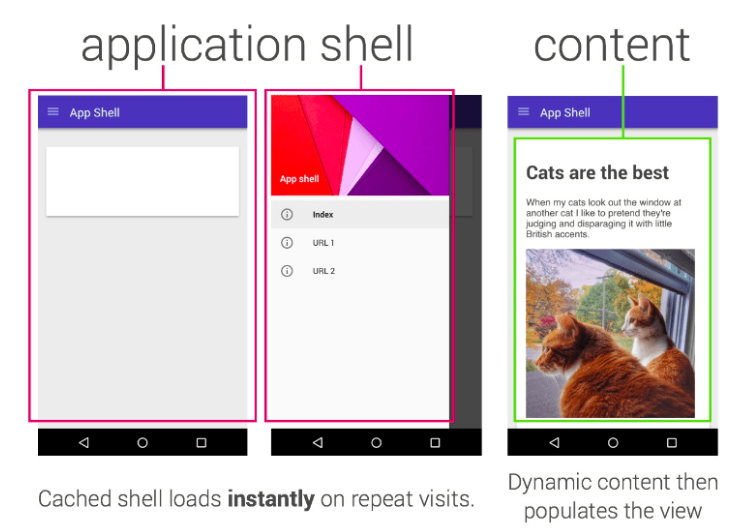
\includegraphics[scale=0.75]{img/appShell.png}
	\caption{Application shell}
	\label{fig:appShell}
\end{figure}
Zoals je ziet op de afbeelding heb je in de application shell het minimum dat je wil tonen aan de gebruiker. Je hebt een basis. Wanneer je de app ook bezoekt, dit zal altijd hetzelfde zijn. Aangezien hier geen (of weinig) verandering is kan je dit lokaal opslaan (cachen). Het dynamisch gedeelte, het artikel, wordt wel via het netwerk geladen. Dit gedeelte, de inhoud, is niet altijd hetzelfde en zal vaak veranderen. Het is dus niet nodig dit lokaal op te slaan. Als er toch updates gedaan worden aan bestanden van de app shell zal de progressive web app dit zien. De volgende keer dat de gebruiker online is zal de app de oude bestanden vervangen door de nieuwe. Als ontwikkelaar is het belangrijk op voorhand te kijken welke bestanden je gaat cachen en welke niet.
Belangrijke voorwaarden voor de app shell 
\begin{itemize}  
	\item Snel laden
	\item Zo weinig mogelijk data gebruiken
	\item Statische bestanden gebruiken van de lokale cache
	\item Inhoud en navigatie scheiden
\end{itemize}

Dit is een voorbeeld van een app shell waarbij het sw.js bestand wordt gecached. 
\lstdefinelanguage{JavaScript}{
	morekeywords={typeof, new, true, false, catch, function, return, null, catch, switch, var, if, in, while, do, else, case, break},
	morecomment=[s]{/*}{*/},
	morecomment=[l]//,
	morestring=[b]",
	morestring=[b]'
}
\lstdefinelanguage{HTML5}{
	language=html,
	sensitive=true, 
	alsoletter={<>=-},
	otherkeywords={
		% HTML tags
		<html>, <head>, <title>, </title>, <meta, />, </head>, <body>,
		<canvas, \/canvas>, <script>, </script>, </body>, </html>, <!, html>, <style>, </style>, ><
	},  
	ndkeywords={
		% General
		=,
		% HTML attributes
		charset=, id=, width=, height=,
		% CSS properties
		border:, transform:, -moz-transform:, transition-duration:, transition-property:, transition-timing-function:
	},  
	morecomment=[s]{<!--}{-->},
	tag=[s]
}

\lstset{%
	% Basic design
	basicstyle={\small\ttfamily},   
	frame=l,
	% Line numbers
	xleftmargin={0.0cm},
	xrightmargin={0.0cm},
	numbers=left,
	stepnumber=1,
	firstnumber=1,
	numberfirstline=true,
	% Code design   
	keywordstyle=\color{blue}\bfseries,
	commentstyle=\color{gray}\ttfamily,
	ndkeywordstyle=\color{editorGreen}\bfseries,
	stringstyle=\color{editorOcher},
	% Code
	language=HTML,
	alsolanguage=JavaScript,
	alsodigit={.:;},
	tabsize=1,
	showtabs=false,
	showspaces=false,
	showstringspaces=false,
	extendedchars=true,
	breaklines=true,        
	% Support for German umlauts
	literate=%
	{Ö}{{\"O}}1
	{Ä}{{\"A}}1
	{Ü}{{\"U}}1
	{ß}{{\ss}}1
	{ü}{{\"u}}1
	{ä}{{\"a}}1
	{ö}{{\"o}}1
}

	\begin{lstlisting}
<!DOCTYPE html>
<html>
<head>
<meta charset="utf-8">
<title>App Shell</title>
<link rel="manifest" href="/manifest.json">
<meta http-equiv="X-UA-Compatible" content="IE=edge">
<meta name="viewport" content="width=device-width, initial-scale=1.0">
<link rel="stylesheet" type="text/css" href="styles/inline.css">
</head>

<body>
<header class="header">
<h1 class="header__title">App Shell</h1>
</header>

<nav class="nav"></nav>

<main class="main"></main>

<div class="dialog-container"></div>

<div class="loader">
<!-- Show a spinner or placeholders for content -->
</div>

<script src="app.js" async></script>
<script>
if ('serviceWorker' in navigator) {
navigator.serviceWorker.register('/sw.js').then(function(registration) {
// Registration was successful
console.log('ServiceWorker registration successful with scope: ', registration.scope);
}).catch(function(err) {
// registration failed :(
console.log('ServiceWorker registration failed: ', err);
});
}
</script>
</body>
</html>
	\end{lstlisting}


Na het creëren van je progressive web app kan je deze laten auditeren door lighthouse. Je progressive web app krijgt een rapport speciaal voor jou opgemaakt. Je krijgt hier een score (op 100) op verschillende punten). Het rapport toont ook waar je nog dingen kunt verbeteren.
\begin{figure}[h]
	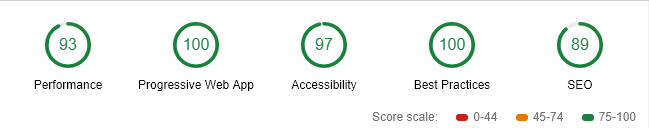
\includegraphics[scale=1]{img/audit.png}
	\caption{Audit progressive webapp}
	\label{fig:audit}
\end{figure}

\begin{itemize}  
	\item Performance: Dit toont hoe goed je huidige app presteert. bv: hoe snel laad de pagina
	\item Progressive web app: In welke mate voldoet de app aan de checklist waaraan een progressive web app moet voldoen. bv: is er een pictogram voor het homescreen
	\item Accessibility: Hoe toegankelijk is je app. bv: kleurencontrast op pagina
	\item Best practices: Hou je je aan de best practices omtrent het schrijven van een web app. bv: geen error logs in de console
	\item SEO: Is je pagina optimaal voor zoekmachines
\end{itemize}



\section{Probleemstelling en Onderzoeksvragen}
\label{sec:onderzoeksvragen}

%% TODO:
%% Uit je probleemstelling moet duidelijk zijn dat je onderzoek een meerwaarde
%% heeft voor een concrete doelgroep (bv. een bedrijf).
%%
%% Wees zo concreet mogelijk bij het formuleren van je
%% onderzoeksvra(a)g(en). Een onderzoeksvraag is trouwens iets waar nog
%% niemand op dit moment een antwoord heeft (voor zover je kan nagaan).

Als bedrijf wil je gemakkelijke gevonden worden door iedereen. Wat voor bedrijf je ook hebt, of je nu spelletjes maakt online, of je nu een bakkerij hebt of een groentenwinkel, een groot bedrijf met honderden werknemers of een eenmanszaak. Als potentiële klanten iets zoeken wat jij aanbiedt, dan wil je dat ze u zo snel en makkelijk mogelijk kunnen vinden. Maar hoe kan je dit het best doen? 

Hulpvragen:
\begin{itemize}  
	\item Investeer je als bedrijf het beste in native of in progressive web apps
\end{itemize}



\section{Opzet van deze bachelorproef}
\label{sec:opzet-bachelorproef}

%% TODO: Het is gebruikelijk aan het einde van de inleiding een overzicht te
%% geven van de opbouw van de rest van de tekst. Deze sectie bevat al een aanzet
%% die je kan aanvullen/aanpassen in functie van je eigen tekst.

De rest van deze bachelorproef is als volgt opgebouwd:

In Hoofdstuk~\ref{ch:methodologie} wordt de methodologie toegelicht en worden de gebruikte onderzoekstechnieken besproken om een antwoord te kunnen formuleren op de onderzoeksvragen.

%% TODO: Vul hier aan voor je eigen hoofstukken, één of twee zinnen per hoofdstuk

In Hoofdstuk~\ref{ch:conclusie}, tenslotte, wordt de conclusie gegeven en een antwoord geformuleerd op de onderzoeksvragen. Daarbij wordt ook een aanzet gegeven voor toekomstig onderzoek binnen dit domein.

